\documentclass[ignorenonframetext,xcolor=x11names]{beamer}

\input{../common.preamble.beamer.tex}
 
\title{Business 4720 - Class 6}

\subtitle{Data Management in Python using Pandas}

\begin{document}

\begin{frame}{}
  \titlepage
  \footnotesize
  \input{../license.tex}
\end{frame}

\section{Introduction}

\begin{frame}{This Class}

\begin{block}{What You Will Learn:}
\begin{itemize}
  \item Introduction to Python
  \item Introduction to the the Numpy package
  \item Introduction to the Pandas package
\end{itemize}
\end{block}
\end{frame}

\section{R}

\begin{frame}{Intro to Python}
\begin{block}{What is Python?}
\begin{itemize}
    \item Readability and simplicity
    \item Dynamic typing enhancing flexibility
    \item Extensive libraries
    \item Procedural, object-oriented, and functional programming
    \item Widely used in data analysis, AI, scientific computing, etc.
    \item Easy to learn
    \item Active community support
\end{itemize}
\end{block}
\vspace{3mm}
\textbf{Intro Tutorial:} \\
\url{https://python.swaroopch.com/} \\
\url{https://github.com/swaroopch/byte-of-python/releases/}
\end{frame}


\begin{frame}{Running Python}
\begin{enumerate}
    \item Interactive Python Shell (command line)
    \item Jupyter Notebooks
    \item PyCharm IDE
\end{enumerate}
\end{frame}

\begin{frame}{Interactive Python Shell}
\begin{itemize}
    \item Similar to the R shell
    \item Type ''python'' to launch Python interpreter
    \item Prompt is ''> > >'', type {\footnotesize\colorbox{lightgray}{ENTER}} to execute a command
    \item Use \texttt{quit()} to exit
    \item Use the {\footnotesize\colorbox{lightgray}{up-arrow}} key to retrieve earlier commands.
    \item Use the {\footnotesize\colorbox{lightgray}{TAB}} key to auto-complete a command.
    \item The Ubuntu terminal uses {\footnotesize\colorbox{lightgray}{SHIFT-CTRL-X}}, {\footnotesize\colorbox{lightgray}{SHIFT-CTRL-C}}, {\footnotesize\colorbox{lightgray}{SHIFT-CTRL-V}} for cut/copy/paste.
    \item \textbf{Tip}: Use a notepad app to assemble commands and to keep results
\end{itemize}
\end{frame}

\begin{frame}{Interactive Python Shell}
\centering
\includegraphics[width=\textwidth]{screen3.png}
\end{frame}

\begin{frame}{Jupyter Notebooks}
\begin{itemize}
    \item Interactive computing environment
    \item Notebook Interface
	\item Combine executable code, text, visualizations
	\item Create and share documents with live code, equations, and explanatory text
	\item Collaborative editing of notebooks (on web-based services)
	\item Popular for Python, but can handle other languages
\end{itemize}
\end{frame}

\begin{frame}{JupyterLabs Desktop}
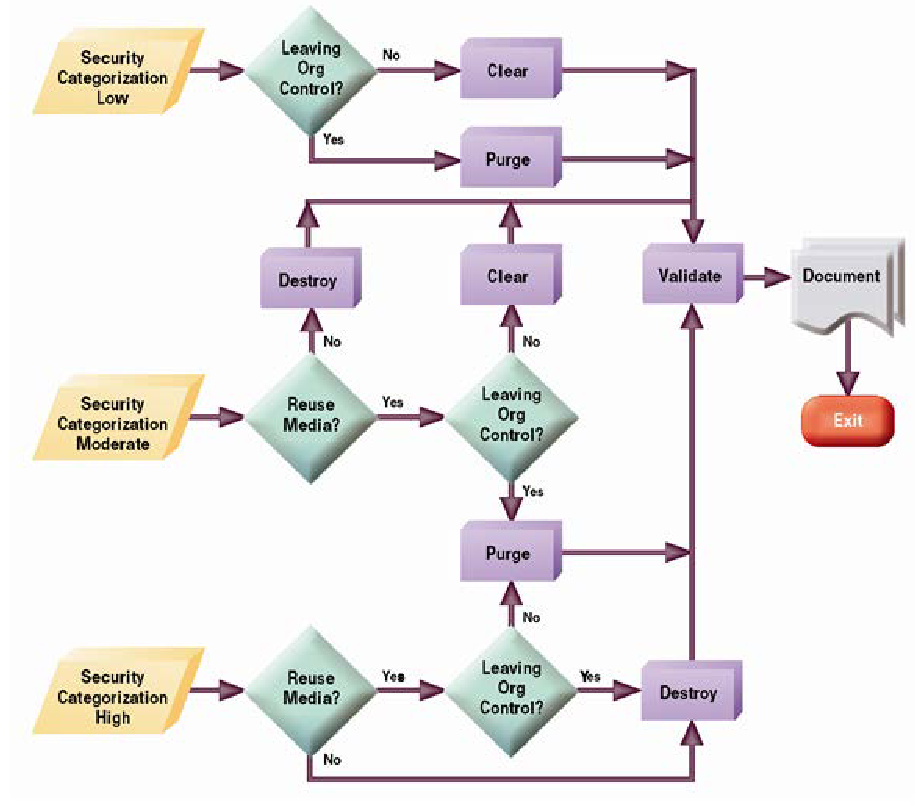
\includegraphics[width=\textwidth]{screen1.png}
\end{frame}

\begin{frame}{JupyterLabs Desktop}

\includegraphics[width=\textwidth]{screen2.png}
\end{frame}

\begin{frame}{Jupyter Notebooks}
\begin{itemize}
  \item ''Kernel'' is the Python interpreter and environment that runs your code
  \item Enter code into empty cell
  \item Press \colorbox{lightgray}{CTRL-ENTER} to execute a cell
  \item Merge, split, move, copy, delete cells
  \item Save, import, export notebooks
\end{itemize}
\end{frame}

\begin{frame}{PyCharm IDE}
\begin{itemize}
   \item When working with multiple Python files in your project
   \item Useful for \emph{programming} (defining functions, classes; using control structures, etc.) rather than just \emph{scripting} (executing a few Python commands one after the other)
   \item Contains built-in debugging tools
\end{itemize}
\end{frame}

\begin{frame}{PyCharm IDE}
\centering
\includegraphics[height=2.5in]{screen4.png}
\end{frame}

\begin{frame}[fragile]{Basic Python}
Python knows math:
\footnotesize
\begin{pythoncode}
# Addition
2 + 2
# Exponentiation
2**4
# Integer division
13 // 3
-13 // 3
# Modulus (remainder)
13 % 3
-25.5 % 2.25
# Comparisons
3 < 5
3 > 5
3 == 5
# Logical and, or, not operators
(3 < 5) and (4 < 2)
(3 < 5) or not (4 < 2)
\end{pythoncode}
\end{frame}


\begin{frame}[fragile]{Basic Python}
String formatting methods:
\footnotesize
\begin{pythoncode}
# Define some variables
age = 19
name = 'Malina'

# Print them in different ways.
# Pick your favourite and stick with it.
print('{0} is {1} years old'.format(name, age))
print('{name} is {age} years old'.format(name=name,age=age))
print('{} is {} years old'.format(name, age))
print(f'{name} is {age} years old')
print(name+' is '+str(age)+' years old')
\end{pythoncode}
\end{frame}

\begin{frame}[fragile]{Basic Python}
Backslashes split and continue lines:
\footnotesize
\begin{pythoncode}
print('This is a very long \
string and needs a second line')
i = \
5
print(i)
\end{pythoncode}
\end{frame}

\begin{frame}[fragile]{Python Strings}
Python knows strings:

\begin{pythoncode}
language = 'Innuktitut'

# Check the start of a string
if language.startswith('Innu'):
    print('Yes, the string starts with "Innu"')
    
# Check if letter contained in string
if 'u' in language:
    print('Yes, it contains the string "u"')
    
# Find the index of a string in another string
# Returns -1 if not found
if language.find('nuk') != -1:
    print('Yes, it contains the string "nuk"')
\end{pythoncode}

Note the colon and the indent of exactly 4 significant spaces!
\end{frame}

\begin{frame}[fragile]{Python Strings}

Joining and splitting strings with a delimiter:

\begin{pythoncode}
# Join a list of strings with a delimiter
delimiter = '_*_'
mylist = ['Nain', 'Hopedale', 'Makkovik', 'Rigolet']
mystring = delimiter.join(mylist)
print(mystring)

# Split a string on a delimiter
thelist = mystring.split(delimiter)
print(thelist)
\end{pythoncode}
\end{frame}

\begin{frame}[fragile]{Lists}
Lists are ordered collections of items:
\begin{pythoncode}
# Define list (Inuit deities)
gods = ['Sedna', 'Nanook', 'Akna', 'Pinga']

# Length of a list
len(gods)
# Iterate over items
for item in gods:
    print(item, end=' ')

# Append to a list
gods.append('Amaguq')
# Sort a list
gods.sort()
# Retrieve items from list
olditem = gods[0]
# Delete item in list
del gods[0]
\end{pythoncode}

Note the colon and the indent of exactly 4 significant spaces!

\end{frame}

\begin{frame}[fragile]{Tuples}
Tuples are immutable:

\begin{pythoncode}
# Define a tuple (Inuit Nunangat)
regions = ('Inuvialuit', 'Nunavut', 'Nunavik', 'Nunatsiavut')

# Length of a tuple
len(regions)

# Create a tuple of tuples, NOT flattened
more_regions = ('Kalaallit', 'Inupiaq', regions)

# Retrieve element 1 of element 3 in tuple
more_regions[2][1]
\end{pythoncode}
\end{frame}

\begin{frame}[fragile]{Dictionaries}
\begin{itemize}
  \item Key--value pairs
  \item Associative arrays
  \item Map
\end{itemize}

\begin{pythoncode}
# Define a dict (largest citites)
c = {
    'Inuvialuit': 'Inuvik',
    'Nunavut': 'Iqaluit',
    'Nunavik': 'Kuujjuaq',
    'Nunatsiavut': 'Nain' 
}
# Get the list of keys
list(c.keys())
# Get the list of values
list(c.values())

# Number of entries in dict
len(c)
\end{pythoncode}
\end{frame}

\begin{frame}[fragile]{Dictionaries \small [cont'd]}
\begin{pythoncode}
# Retrieve a value for a key:
c['Nunavik']

# Delete a key-value pair
del c['Nunavut']

# Add a key-value pair
c['Nunavut'] = 'Iqaluit'

# Check for existence of a key
if 'Nunavut' in c:
    print("\nNunavut's largest city is", c['Nunavut'])
\end{pythoncode}
\end{frame}

\begin{frame}{Structured Data Types}
\begin{block}{Important}
\begin{itemize}
  \item Indexing begins at 0 (different from R!)
  \item Can contain any data type
\end{itemize}
\end{block}

\begin{block}{Sequences}
\begin{itemize}
  \item List, tuples, strings are sequences
  \item Membership tests using \texttt{in} or \texttt{not in}
  \item Indexing and slicing
\end{itemize}
\end{block}
\end{frame}

\begin{frame}[fragile]{Slicing}
\footnotesize
\begin{pythoncode}
regions = ('Inuvialuit', 'Nunavut', 
           'Nunavik', 'Nunatsiavut')
language = 'Innuktitut'

# Slicing on a tuple
regions[1:3]
regions[2:]
regions[1:-1]
regions[:]

# Slicing with step size
regions[::1]
regions[::2]
regions[::3]
regions[::-1]
\end{pythoncode}
\end{frame}

\begin{frame}{Hands-On Exercises}
\begin{block}{Lists}
\begin{enumerate}
    \item Create a list containing the numbers 1 to 10. Use list slicing to create a sublist with only the even numbers.
    \item Using a \texttt{for} loop, sum all the items in the list.
    \item Using a \texttt{for} loop, iterate over the list and print each number squared.
    \item Write a program to append the square of each number in the range [1:5] to a new list.
\end{enumerate}
\end{block}
\end{frame}
\begin{frame}{Hands-On Exercises}
\begin{block}{Tuples}
\begin{enumerate}
    \item Create a tuple with different data types (string, int, float).
    \item Demonstrate how tuples are immutable by attempting to change its first element.
\end{enumerate}
\end{block}

\begin{block}{Dictionaries}
\begin{enumerate}
    \item Create a nested dictionary and demonstrate accessing elements at various levels. A nested dictionary is one in which the values themselves are also dictionaries.
\end{enumerate}
\end{block}
\end{frame}

\begin{frame}{Numerical Data in Python with NumPy}
\begin{block}{What is Numpy?}
\begin{itemize}
    \item High-performance scientific computing and data analysis.    
    \item Multidimensional arrays
    \item Comprehensive mathematical function library
    \item Foundational package for other scientific libraries like SciPy, Pandas, Matplotlib, scikit-learn, scikit-image, etc.
\end{itemize}
\end{block}

\begin{block}{Intro Tutorials}
\begin{itemize}
\item \href{https://numpy.org/doc/stable/user/quickstart.html}{NumPy Quickstart} \\ 

\item \href{https://numpy.org/doc/stable/user/absolute_beginners.html}{NumPy for Absolute Beginners}
\end{itemize}
\end{block}
\end{frame}

\begin{frame}[fragile]{NumPy Array}
N-Dimensional Array, type ''\texttt{ndarray}'' \\

\begin{pythoncode}
# Import the numpy package
import numpy as np

# Create an array
a = np.arange(15).reshape(3, 5)

# Examine its properties
a.shape
a.ndim
a.dtype.name
a.size
\end{pythoncode}
\end{frame}

\begin{frame}[fragile]{NumPy Basics}

\begin{pythoncode}
# Create an array from Python lists and tuples
b = np.array([(1.5, 2., 3), 
              (4.0, 5., 6)])
print(b)

# Elementwise operations
3 * b
b + 5
np.sqrt(b)

# NumPy array functions
np.sum(b)
np.max(b)
# Axis 0 is by column
np.max(b, axis=0)
# Axis 1 is by row
np.max(b, axis=1)
np.std(b, axis=0)
# Transpose
np.transpose(b)
# Cov default by row
np.cov(b)
np.cov(np.transpose(b))
\end{pythoncode}
\end{frame}

\begin{frame}[fragile]{NumPy Basics \small [cont'd]}

\begin{pythoncode}
# Create an array of zeros with shape (3,4)
x = np.zeros((3,4))
print(x)

# Create an array of ones with shape (2,3,4)
y = np.ones((2,3,4))
print(y)
\end{pythoncode}
\end{frame}

\begin{frame}[fragile]{Array Slicing}
\begin{itemize}
    \item Each axis can be sliced using \texttt{[:]} or \texttt{[::]}
\end{itemize}

\begin{pythoncode}
b = np.array([[ 0,  1,  2,  3],
              [10, 11, 12, 13],
              [20, 21, 22, 23],
              [30, 31, 32, 33],
              [40, 41, 42, 43]])

# One element              
b[2, 3]
# Multiple rows, one column
b[0:5, 1]
# Every other row up to 4, one column
b[0:5:2, 1]
# All rows, columns 1 and then every other
b[:, 1::2]
# Two rows, all columns
b[1:3, :]
# Last row
b[-1]
# Last column
b[:,-1]
\end{pythoncode}
\end{frame}

%\begin{frame}[fragile]{Array Slicing \& Iterators}
%\footnotesize
%\begin{pythoncode}
%c = np.array([[[  0,  1,  2],
               %[ 10, 12, 13]],
              %[[100, 101, 102],
               %[110, 112, 113]]])
               
%print(c.shape)
%print(c[1, ...])
%print(c[1, : , : ])
%print(c[..., 2])
%print(c[: , : , 2])
%print(c[..., : , 1])

\end{pythoncode}
\end{frame}

\begin{frame}[fragile]{Array Reshaping}

\begin{pythoncode}
# Create 3x4 array of random numbers
a = np.floor(10 * np.random.random((3, 4)))

a.shape
a.flatten()
a.reshape(6, 2)
a.T
a.T.shape

# Create another 3x4 array of random numbers
b = np.floor(5 * np.random.random((3, 4)))
# Vertical stacking
np.vstack((a, b))
# Horizontal stacking
np.hstack((b, a))

# Iterate over rows
for row in b:
    print(row)
    
# Iterate over all elements
for element in b.flat:
    print(element)
\end{pythoncode}
\end{frame}

\begin{frame}[fragile]{Array Indexing with Boolean Arrays}

\begin{pythoncode}
a = np.array([[1,  2,  3,  4], 
              [5,  6,  7,  8], 
              [9, 10, 11, 12]])

# Are entries less than 5?
a < 5
# Entries that are less than 5
a[a < 5]

# Are entries even?
a%2 == 0
# Entries that are even
a[a%2 == 0]
\end{pythoncode}
\end{frame}              

%\begin{frame}[fragile]{Unique Elements and Counts}
%\footnotesize
%\begin{pythoncode}
%a = np.array([11, 11, 12, 13, 14, 15, 16, 
              %17, 12, 13, 11, 14, 18, 19, 20])
             
%print(np.unique(a))

%values, indices = np.unique(a, return_index=True)
%print(list(zip(values, indices)))

%values, counts = np.unique(a, return_counts=True)
%print(list(zip(values, counts)))
%\end{pythoncode}
%\end{frame}

\begin{frame}{Hands-On Exercises}
\begin{enumerate}
   \item Create a four-dimensional array with random numbers in the shape indicated by the last four digits of your student number (if your student number contains a 0, use a 1 instead)
   \item Construct a new array by swapping the first half of rows (axis 0) with the second half of rows (axis 0)
   \item Calculate all covariance matrices formed by the last two axes of your array. \emph{Tip:} Iterate over the first two axes/dimensions with a \texttt{for} loop
   \item Subtract the mean of the array from each element in the array (mean normalization)
   \item Select all elements that are greater than the overall mean
   \item Sort the selected elements from the previous step in ascending order
\end{enumerate}
\end{frame}


\begin{frame}{Data Management with Pandas}
\begin{block}{What is Pandas?}
\begin{itemize}
    \item Open-source library for data analysis
    \item High-performance, easy-to-use data structures and data analysis tools    
    \item Can handle tabular data, time series, matrix data, etc.
    \item Tools for data cleaning, transformation, and preparation    
    \item Importing data from CSV, Excel, SQL databases, etc.    
    \item Functions for aggregating, pivoting, joining, and sorting data
\end{itemize}
\end{block}
\vspace{5mm}
\textbf{Intro Tutorial}: \href{http://pandas.pydata.org/docs/user_guide/10min.html}{10 Minutes to Pandas}
\end{frame}

%\begin{frame}[fragile]{Pandas Series}
%\begin{itemize}
    %\item 1-Dimensional \emph{labelled} array
    %\item Axis labels are called \emph{index}
%\end{itemize}
%\footnotesize
%\begin{pythoncode}
%# Import the Pandas package
%import pandas as pd

%# Series from random numbers
%s = pd.Series(np.random.randn(5))
%print(s.index)

%# Series with labels from random numbers
%s = pd.Series(np.random.randn(5), 
              %index=["a", "b", "c", "d", "e"])
%print(s.index)

%# Series from dict
%d = {"a": 0.0, "b": 1.0, "c": 2.0}
%pd.Series(d)

%# Series from dict and reorder entries
%# Produces NaN for index d
%pd.Series(d, index=["b", "c", "d", "a"])
%\end{pythoncode}
%\end{frame}

%\begin{frame}[fragile]{Pandas Series \small [cont'd]}
%\footnotesize
%\begin{pythoncode}
%# Series behave like an ndarray
%s.iloc[0]
%s.iloc[:3]
%s[s > s.median()]
%s.iloc[[4, 3, 1]]
%np.exp(s)

%# Series behave like a dict
%s['a'])
%s['e'])
%'e' in s
%'f' in s
%\end{pythoncode}
%\end{frame}

\begin{frame}[fragile]{Pandas Dataframe}
\begin{itemize}
   \item 2-dimensional
   \item Row labels are called \emph{index}
   \item Columns may have different data types
   %\item A dict of multiple pandas series 
\end{itemize}
\footnotesize
\begin{pythoncode}
# Create a dict of two Series
d = {
    "col1": pd.Series([1.0, 2.0, 3.0], 
                index=['a', 'b', 'c']),
    "col2": pd.Series([1.0, 2.0, 3.0, 4.0], 
                index=['a', 'b', 'c', 'd'])
}

# Create a dataframe from dict
df = pd.DataFrame(d)
\end{pythoncode}
\end{frame}

\begin{frame}[fragile]{Pandas Dataframe -- Basic Information}
\footnotesize
\begin{pythoncode}
# Dimensions (rows, columns)
df.shape

# Row labels (index)
list(df.index)
# Column labels
list(df.columns)

# Information about columns and data types
df.info()

# First few rows
df.head()
# Last few rows
df.tail()

# Summary of data
df.describe()
\end{pythoncode}
\end{frame}

%\begin{frame}[fragile]{Pandas Dataframe Columns}
%\footnotesize
%\begin{pythoncode}
%# Access a column
%df['col1']

%# Create a new calculated column
%df['col3'] = df['col1'] * df['col2']

%# Create another new calculated column using 'assign'
%df = df.assign(col4 = df['col1'] * np.sqrt(df['col2']))
%\end{pythoncode}
%\end{frame}

%\begin{frame}[fragile]{Dataframe Indexing}
%\renewcommand{\arraystretch}{1.5}
%\centering
%\small

%\begin{tabular}{l|l|l} \hline
%Select column & \texttt{df[col]} & Series \\
%Select row by label & \texttt{df.loc[label]}  & Series \\
%Select row by integer location & \texttt{df.iloc[loc]} & Series \\
%Slice rows & \texttt{df[::]} & DataFrame \\
%Select rows by boolean vector & \texttt{df[bool]} & DataFrame \\ \hline
%\end{tabular}
%\end{frame}

\begin{frame}[fragile]{Pandas Dataframe -- Indexing}
\begin{pythoncode}
# Select one column
df['col1']

# Select multiple columns (list of columns)
df[['col1', 'col2']]

# Select rows by label, returns Series
df.loc['a']

# Select single row by number
df.iloc[2]

# Select single column by number
df.iloc[:,1]

# Select rows 0 to 3, columns 0 to 1
df.iloc[0:4:2, 0:2] 

# Select every other row 0 to 3
df[0:4:2]

# Select rows by boolean array
df[df['col1'] > 2]
\end{pythoncode}

\end{frame}

\begin{frame}[fragile]{Pandas Dataframe -- Operations}
%\begin{itemize}
    %\item Data is aligned on column labels and row indices
%\end{itemize}

%df = pd.DataFrame(np.random.randn(10, 4), 
                  %columns=["A", "B", "C", "D"])
%df2 = pd.DataFrame(np.random.randn(7, 3), 
                   %columns=["A", "B", "C"])
%df + df2

\begin{pythoncode}
# Elementwise operators
df * 5 + 2
1/df
df**4

# Transpose
df.T

# Using Numpy functions on Pandas data frames
np.exp(df)
np.sum(df[['col1', 'col2']], axis=1)
\end{pythoncode}
\end{frame}

%\begin{frame}[fragile]{Pandas Dataframe}
%\footnotesize
%\begin{pythoncode}
%# Boolean reductions
%(df > 0).all()
%(df > 0).any()
%(df > 0).any().any()

%# NaN's are not the same
%df.iloc[0,0] = np.nan
%(df+df == df*2).all()
%(df + df).equals(df*2)
%\end{pythoncode}
%\end{frame}

%\begin{frame}[fragile]{Descriptive Statistics, Aggregation, \& Strings}

%\begin{pythoncode}
%# Descriptive statistics
%# By column
%df.mean(axis=0)
%# By row
%df.mean(axis=1, skipna=False)

%# Aggregation with 'agg', by column
%df.agg(['sum', 'mean', 'std'], axis=0)

%# Sort values by columns
%df.sort_values(by=['col1', 'col2'])

%# Find 3 rows with smallest or largest values by column
%df.nsmallest(3, 'col1')
%df.nlargest(3, 'col2')
%\end{pythoncode}
%\end{frame}

\begin{frame}[fragile]{Pandas Dataframe -- Selection with Query}

\begin{pythoncode}
df = pd.DataFrame(np.random.rand(10, 3), 
           columns=['a', 'b', 'c'])
                  
# Pure python
df[(df['a'] < df['b']) & (df['b'] < df['c'])]

# Shorter with Query
df.query('(a < b) & (b < c)')
df.query('a < b & b < c')
df.query('a < b and b < c')
df.query('a < b < c')
\end{pythoncode}
\end{frame}

%\begin{frame}[fragile]{Selection with Query \small [cont'd]}
%\footnotesize
%\begin{pythoncode}
%df = pd.DataFrame({'a': list('aabbccddeeff'), 
                   %'b': list('aaaabbbbcccc'),
                   %'c': np.random.randint(5, size=12),
                   %'d': np.random.randint(9, size=12)})      
                   
%# Pure Python versus Query
%df[df['a'].isin(df['b'])]  
%df.query('a in b')  

%df[~df['a'].isin(df['b'])] 
%df.query('a not in b')     

%df[df['b'].isin(df['a']) & (df['c'] < df['d'])]          
%df.query('a in b and c < d') 

%df[df['b'].isin(["a", "b", "c"])]
%df.query('b == ["a", "b", "c"]')    

%df[df['c'].isin([1, 2])]
%df.query('[1, 2] in c')      
%\end{pythoncode}
%\end{frame}

%\begin{frame}[fragile]{Duplicate Data}
%\footnotesize
%\begin{pythoncode}
%df2 = df.copy()

%df2.duplicated(['a', 'b'])
%df2.drop_duplicates(['a', 'b'], keep='last')
%df2.drop_duplicates(['a', 'b'], keep='first')
%\end{pythoncode}
%\end{frame}

%\begin{frame}[fragile]{Reading Data into Pandas}
%\begin{itemize}
    %\item Wide variety of format: CSV, JSON, Excel, SQL, \ldots
    %\item \url{https://pandas.pydata.org/docs/user_guide/io.html#}
%\end{itemize}
%\end{frame}

\begin{frame}{Easy Pandas -- Example Dataset}
\begin{itemize}
  \item Government of Canada, Open Government Portal
  \item Fuel Consumption Ratings -- Battery-electric vehicles -- 2012--2023
  \item \href{https://open.canada.ca/data/en/dataset/98f1a129-f628-4ce4-b24d-6f16bf24dd64}{https://open.canada.ca/data/en/dataset/98f1a129-f628-4ce4-b24d-6f16bf24dd64}
\end{itemize} 

\vspace{\baselineskip}
\centering
\footnotesize

	\begin{tabular}{|l|l|} \hline
	  {\bf Column} & {\bf Data Type} \\ \hline \hline
	  Make & Categorical (string) \\ 
	  Model & Categorical (string) \\
	  Year & Numeric \\
	  Category & Categorical (string)\\
	  City & Numeric \\
	  Hwy & Numeric \\
	  Comb & Numeric \\
	  Range & Numeric \\ \hline
	\end{tabular}
\end{frame}

\begin{frame}[fragile]{Easy Pandas -- Reading CSV Files}
\begin{pythoncode}
# Import pandas 
import pandas as pd

# Read CSV into a Pandas data frame
data = pd.read_csv('https://evermann.ca/busi4720/fuel.csv')

# Basic information about data
data.shape
list(data.columns)
data.info()
data.describe()
\end{pythoncode}
\end{frame}

\begin{frame}[fragile]{Easy Pandas -- Filtering}
\begin{pythoncode}
# Filter values
data.query('Make=="Ford" & Year==2023')
\end{pythoncode}

\vspace{\baselineskip}
\begin{columns}
\begin{column}{.5\textwidth}
Equivalent in R:
\begin{Rcode}
data |> 
  filter(Make=='Ford', 
         Year==2023) |> 
  print()
\end{Rcode}
\end{column}
\begin{column}{.5\textwidth}
Equivalent in SQL:
\begin{sqlcode}
SELECT * 
   FROM data 
   WHERE Make=='Ford' AND 
         Year==2023;
\end{sqlcode}
\end{column}
\end{columns}
\end{frame}

\begin{frame}[fragile]{Easy Pandas -- Selecting Columns}

\begin{pythoncode}
# Filter values and select columns
data.query('Make=="Ford" & Year==2023') \
    [['Model', 'Category', 'Range']]
\end{pythoncode}

\vspace{\baselineskip}

\begin{columns}
\begin{column}{.5\textwidth}
Equivalent in R
\begin{Rcode}
data |> 
  filter(Make=='Ford', 
         Year==2023) |> 
  select(Model, Category, 
            Range) |>
  print()
\end{Rcode}
\end{column}
\begin{column}{.5\textwidth}
Equivalent in SQL:

\begin{sqlcode}
SELECT Model, Category, Range 
   FROM data 
   WHERE Make=='Ford' AND 
         Year==2023;
\end{sqlcode}
\end{column}
\end{columns}
\end{frame}

\begin{frame}[fragile]{Easy Pandas -- Create New Columns}

\begin{pythoncode}
# Filter values, create new calculated column and select cols
data.query('Make=="Ford" & Year==2023') \
  .assign(HwyRange = data['Range']*data['Comb']/data['Hwy']) \
  [['Model', 'Category', 'Range', 'HwyRange']]
\end{pythoncode}

\vspace{\baselineskip}

\begin{columns}
\begin{column}{.5\textwidth}
Equivalent in R:
\begin{Rcode}
data |> 
  filter(Make=='Ford', 
         Year==2023) |> 
  mutate(HwyRange=
            Range*Comb/Hwy) |>
  select(Model, Category, 
         Range, HwyRange) |>
  print()
\end{Rcode}
\end{column}
\begin{column}{.5\textwidth}
Equivalent in SQL:

\begin{sqlcode}
SELECT Model, Category, Range, 
  (Range*Comb)/Hwy AS HwyRange 
   FROM data 
   WHERE Make=='Ford' AND 
         Year==2023;
\end{sqlcode}
\end{column}
\end{columns}
\end{frame}

\begin{frame}[fragile]{Easy Pandas -- Renaming Columns}

\begin{pythoncode}
# Filter values, create two new calculated columns,
# rename a column, and select columns
data.query('Make=="Ford" & Year==2023') \
  .assign(HwyRange = data['Range']*data['Comb']/data['Hwy']) \
  .assign(CityRange = data['Range']*data['Comb']/data['City']) \
  .rename(columns={'Range': 'CombRange'}) \
  [['Model', 'Category', 'CombRange', 'CityRange', 'HwyRange']]
\end{pythoncode}

\vspace{\baselineskip}

\begin{columns}
\begin{column}{.5\textwidth}

Equivalent in R:
\begin{Rcode}
data |> 
  filter(Make=='Ford', 
         Year==2023) |> 
  mutate(HwyRange = 
     Range * Comb / Hwy) |>
  mutate(CityRange = 
     Range * Comb / City) |>
  rename(CombRange = Range) |>
  select(Model, Category, 
         CombRange, CityRange, 
         HwyRange) |>
  print()
\end{Rcode}
\end{column}
\begin{column}{.5\textwidth}
Equivalent in SQL:
\begin{sqlcode}
SELECT Model, Category, 
      Range AS CombRange,
      (Range * Comb) / Hwy 
          AS HwyRange, 
      (Range * Comb) / City 
          As CityRange
   FROM data 
   WHERE Make=='Ford' AND 
         Year==2023;
\end{sqlcode}
\end{column}
\end{columns}
\end{frame}

\begin{frame}[fragile]{Easy Pandas -- Distinct Values}
\begin{pythoncode}
# Find distinct values
data[['Make', 'Model']].drop_duplicates()
\end{pythoncode}

\vspace{\baselineskip}
\begin{columns}
\begin{column}{.5\textwidth}
Equivalent in R:

\begin{Rcode}
data |> 
  distinct(Make, Model) |>
  print()
\end{Rcode}
\end{column}
\begin{column}{.5\textwidth}
Equivalent in SQL:

\begin{sqlcode}
SELECT DISTINCT Make, Model 
  FROM data;
\end{sqlcode}
\end{column}
\end{columns}
\end{frame}

\begin{frame}[fragile]{Easy Pandas -- Ordering}
\begin{pythoncode}
# Filter values, order by values of two columns
# and select columns
data.query('Make=="Ford" & Year==2023') \
  .sort_values(['Category', 'Range'], ascending=[True, False]) \
  [['Model', 'Category', 'Range']]
\end{pythoncode}

\vspace{\baselineskip}
\begin{columns}
\begin{column}{.5\textwidth}
Equivalent in R:
\begin{Rcode}
data |> 
  filter(Make=='Ford', 
         Year==2023) |> 
  select(Model, Category, 
         Range) |>
  arrange(Category, 
          desc(Range)) |>
  print()
\end{Rcode}

\end{column}
\begin{column}{.5\textwidth}
Equivalent in SQL:

\begin{sqlcode}
SELECT Model, Category, Range
   FROM data 
   WHERE Make=='Ford' AND 
         Year==2023
   ORDER BY Category ASC, 
            Range DESC;
\end{sqlcode}
\end{column}
\end{columns}
\end{frame}

\begin{frame}[fragile]{Easy Pandas -- Grouping and Summarizing}
\begin{pythoncode}
# Filter values, group the data,
# calculate aggregates of multiple columns
# filter on aggregate data, order by value
# and select certain columns
data.query('Year==2023') \
    .groupby(['Make', 'Category']) \
    .agg(meanCity = ('City', 'mean'),
         meanHwy = ('Hwy', 'mean'),
         meanComb = ('Comb', 'mean'),
         maxRange = ('Range', 'max'),
         nVehicle = ('Model', 'count')) \
    .query('nVehicle > 1') \
    .sort_values(['Category', 'meanComb']) \
    .reset_index() \
    [['Category', 'meanComb', 'Make', 'meanCity', \
      'meanHwy', 'maxRange', 'nVehicle']]
\end{pythoncode}

\end{frame}
\begin{frame}[fragile]{Grouping and Summarizing \small [cont'd]}
\begin{columns}
\begin{column}{.5\textwidth}
Equivalent in R:
\begin{Rcode}
data |> 
  filter(Year==2023) |> 
  group_by(Make, Category) |>
  summarize(
       meanCity = mean(City), 
       meanHwy = mean(Hwy),
       meanComb = mean(Comb),
       maxRange = max(Range),
       nVehicle = n()) |>
  filter(nVehicle > 1) |>
  arrange(Category,meanComb) |>
  relocate(Category,meanComb) |>
  print()
\end{Rcode}
\end{column}
\begin{column}{.5\textwidth}
Equivalent in SQL:

\begin{sqlcode}
SELECT Category, 
       AVG(Comb) AS meanComb,
       Make,
       AVG(City) AS meanCity,
       AVG(Hwy) AS meanHwy,
       MAX(Range) AS maxRange,
       COUNT(*) AS nVehicle
   FROM data 
   WHERE Year==2023
   GROUP BY Make, Category
   HAVING COUNT(*) > 1
   ORDER BY Category ASC, 
            meanComb ASC;
\end{sqlcode}
\end{column}
\end{columns}
\end{frame}

\begin{frame}[fragile]{Advanced Pandas with the Pagila Database}
\begin{pythoncode}
rentals = pd.read_csv(
     'http://evermann.ca/busi4720/rentals.csv')
     
actors = pd.read_csv(
     'https://evermann.ca/busi4720/actors.categories.csv')
     
addresses = pd.read_csv(
     'https://evermann.ca/busi4720/addresses.csv')
\end{pythoncode}
\end{frame}

\begin{frame}[fragile]{Advanced Pandas with the Pagila Database  \small [cont'd]}
Find all films and the actors that appeared in them, ordered by film category and year, for those films that are rated PG:

\scriptsize
\begin{pythoncode}
data = pd.merge(rentals, actors, on='title', 
         suffixes=('_customer', '_actor'), how='outer')
data.query('rating == "PG"') \
    .assign(actor = data['last_name_actor'] + \
                   ', ' + data['first_name_actor']) \
    .rename(columns={'release_year': 'year'}) \
    [['actor', 'title', 'category', 'year']] \
    .drop_duplicates(['actor', 'title', 'category', 'year']) \
    .groupby(['category', 'year', 'title']) \
    ['actor'].apply(list) \
    .reset_index() \
    .sort_values(['category', 'year']) \
\end{pythoncode}
\end{frame}


\begin{frame}[fragile]{Advanced Pandas with the Pagila Database \small [cont'd]}

Find the most popular actors in the rentals in each city:

\scriptsize
\begin{pythoncode}
full_data = pd.merge(rentals, addresses, 
                     left_on='customer_address', 
                     right_on='address_id')
full_data = pd.merge(full_data, actors, on='title', 
                     suffixes=('_customer', '_actor'))
\end{pythoncode}

\begin{pythoncode}
full_data \
   .assign(actor=full_data['last_name_actor'] + ', ' + 
                 full_data['first_name_actor'] ) \
   .groupby(['city', 'actor']) \
   .agg(count = ('title', 'count')) \
   .reset_index() \
   .assign(ranking=lambda df: 
      df.groupby('city')['count']
        .rank(method='min', ascending=False)) \
   .query('ranking <= 3') \
   .sort_values(by=['city', 'ranking', 'actor'])
\end{pythoncode}

\end{frame}

\begin{frame}[fragile]{Advanced Pandas with the Pagila Database \small [cont'd]}

Find the customers who spend the most on rentals, and the number of rentals with the higest total rental payments for each category grouped by rental duration.

\scriptsize
\begin{pythoncode}
full_data \
   .assign(customer=full_data['last_name_customer'] + ', ' + 
                    full_data['first_name_customer'] ) \
   [['customer', 'amount', 'rental_duration', \
     'category', 'phone', 'city']] \
   .groupby(['category', 'rental_duration', 'customer']) \
   .agg(payments =('amount', 'sum'), 
        num_rentals=('amount', 'count')) \
   .reset_index() \
   .assign(ranking=lambda df: \
      df.groupby(['category','rental_duration'])['payments'] \
        .rank(method='min', ascending=False)) \
    .loc[lambda df:  \
         df.groupby(['category', 'rental_duration'])
            ['ranking'].idxmin() ]
\end{pythoncode}
\end{frame}

\begin{frame}[fragile]{Advanced Pandas with the Pagila Database \small [cont'd]}
Get the top 5 and the bottom 5 grossing customers for each quarter.

\footnotesize
\begin{pythoncode}
full_data \
   .assign(customer=full_data['last_name_customer'] + ', ' + 
                    full_data['first_name_customer'],
           q=pd.to_datetime(full_data['rental_date'],utc=True)
                 .dt.to_period("Q"))  \
   [['customer', 'q', 'amount', 'rental_date']] \
   .groupby(['q', 'customer']) \
   .agg(payments=('amount', 'sum')) \
   .reset_index() \
   .drop_duplicates(['customer', 'q', 'payments']) \
   .assign(rank_top = lambda df : 
              df.groupby('q')['payments']
                .rank(method='min', ascending=False),
           rank_bot = lambda df : 
              df.groupby('q')['payments']
              .rank(method='min', ascending=True)) \
    .reset_index() \
    .query('rank_top <= 5 or rank_bot <= 5') \
    .sort_values(by=['q','payments'],ascending=[True,False]) 

\end{pythoncode}
\end{frame}


\begin{frame}[fragile]{Advanced Pandas with the Pagila Database \small [cont'd]}

Find the set of film titles by rental customer and the total number rentals for each customer

\scriptsize
\begin{pythoncode}
full_data \
   .assign(customer=full_data['last_name_customer'] + ', ' + 
                    full_data['first_name_customer']) \
   [['customer', 'title']] \
   .groupby('customer') \
   ['title'].apply(list) \
   .reset_index(name='titles') \
   .assign(rentals = lambda df :
              df['titles'].apply(len) ,
           unique_titles = lambda df :
              df['titles'].apply(lambda x: list(set(x)))) \
   .drop(columns=['titles']) \
   .sort_values(by='customer')

\end{pythoncode}
\end{frame}

\begin{frame}{Hands-On Exercises}
\begin{enumerate}
  \item Find all films with a rating of 'PG'
  \item List all customers who live in Canada (with their address)
  \item Find the average \emph{actual} rental duration for all films
  \begin{itemize}
     \item This requires date arithmetic
  \end{itemize}
  \item Find the average overdue time for each customer
  \begin{itemize}
     \item This requires date arithmetic
  \end{itemize}
  \item List all films that have never been rented
  \item List the names of actors who have played in more than 15 films
\end{enumerate}
\end{frame}

\end{document}


